%%=============================================================================
%% Methodologie
%%=============================================================================

\chapter{\IfLanguageName{dutch}{Methodologie}{Methodology}}%
\label{ch:methodologie}

In dit hoofdstuk stellen we de verwachtingen van MFPOSS vast. Dit doen we zodat het prototype geëvalueerd kan worden zodra het is voltooid. Dit wordt het best gedaan aan de hand van de MoSCoW-methode. Deze methode houdt in dat van tevoren wordt bepaald wat MFPOSS wil van het product, en deze criteria worden verdeeld in de volgende categorieën:

\begin{itemize}
    \item Must have
    \item Should have
    \item Could have
    \item Won't have
\end{itemize}

\section{MoSCoW}

\subsection{Must have}
Voor MFPOSS is het belangrijk dat er eenvoudig te zien is welke berichten vaak voorkomen en welke zelden voorkomen.

\subsection{Should have}
Het is ook de taak van ELK om het leven voor MFPOSS makkelijker te maken zonder dat er te veel extra werk aan besteed moet worden. Het moet dus eenvoudig zijn om elementen aan het dashboard toe te voegen zonder veel programmeerwerk. Het is ook belangrijk dat MFPOSS afwijkingen kan detecteren. Deviatiedetectie kan hierbij goed helpen.

\subsection{Could Have}
Het zou interessant zijn om te onderzoeken of er automatisch meldingen naar MFPOSS kunnen worden gestuurd als ELK iets ongewoons opmerkt.

\subsection{Won't Have}
Een complexe implementatie waaruit te weinig informatie kan worden gehaald. Daarnaast mag het niet te veel extra werk vergen om zaken aan te passen of toe te voegen.

Nadat een prototype is opgesteld voor elke analyser, zal worden beoordeeld of het voldoet aan de vooraf vastgestelde MoSCoW-criteria. Als het prototype niet ten minste aan de "Must have" en "Won't have" criteria voldoet, betekent dit dat het voor MFPOSS niet voldoende is om verder mee te werken. Alle analysers dat overblijven gaan worden vergeleken met elkaar wanneer het aankomt op gemak van gebruik, stijl, prijs en effeicientie.

\Section{Linux}
Een mainframe heeft zoals eerder besproken limitaties dat boven komen doordat het een niche platform is. Dit zou voor problemen kunnen zorgen wanneer het aankomt op support. Gelukkig voor mainframe teams kan de mainframe een Linux server draaien waarop er vandaag de dag meer support is voor de log analysers. Op deze methode omzeilen we niet alleen de limitaties van een mainframe maar geraken we ook terecht in een situatie waar traditionele bedrijven zich ook meestal vinden aangezien een groot deel daarvan Linux servers gebruiken of allesinds toegang kunnen vergrijgen tot één. Ook is dit handig voor bedrijven met meerdere mainframe teams aangezien dat logs zich op verschillende plaatsen kunnen vinden en het niet altijd even eenvoudig is om ze rechstreeks naar de analyser te sturen. Maar als er een Linux server bestaat kan dit dienen als soor landing zone voor alle teams en kan er van hier uit een reproduceerbare methode gevonden worden om alle logs te versturen. Om dit te doen moet er natuurlijk eerst een Linux server oopgesteld worden. 

TO DO: Linux server op mainframe opstellen?
\subsection{Linux op mainframe}

\subsection{Versturen van data}
Nu moet alleen de link gemaakt kunnen worden van de mainframe naar de linux server. Dit gaat gebeuren aan de hand van een JCL job. Die job gaat ervoor zorgen da we de logbestanden kunnen FTPen naar de Linux server en ze meteen in de goeie directory kunnen steken.

\begin{figure}[h]
    \centering
    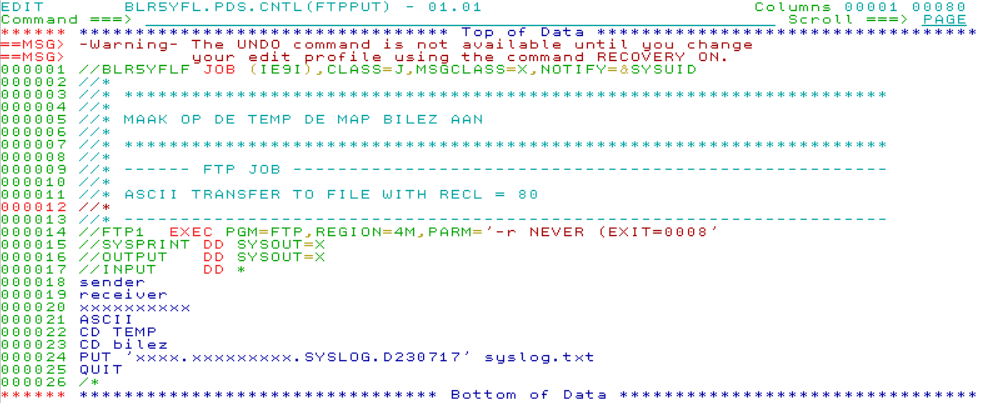
\includegraphics[width=1\linewidth]{bachproef//graphics/FTP JCL.png}
    \caption{Een voorbeeld van hoe een JCL-bestand voor FTP eruit kan zien}
    \label{fig:Een voorbeeld van hoe een JCL-bestand voor FTP eruit kan zien}
\end{figure}

Figuur 4.4 is een voorbeeld van een JCL-taak die bedoeld is om een bestand via FTP naar een bepaalde locatie te verzenden. Regel één is een standaard JCL-regel, waarbij de enige relevante variabelen de naam van de taak en het projectnummer zijn. Er zijn meer opties, maar die vallen buiten de reikwijdte van dit onderzoek. Regels twee tot en met dertien zijn opmerkingen. Regel veertien geeft aan dat dit een FTP-taak is. Vanaf regel achttien beginnen de variabelen en commando's om het bestand succesvol over te brengen:

\begin{itemize}
    \item lijn 18: De naam van het systeem dat het bestand verstuurt.
    \item lijn 19: De naam van het systeem dat het bestand ontvangt.
    \item lijn 20: Het wachtwoord van het ontvangende systeem.
    \item lijn 21: Het formaat van de inhoud van het bestand; voor dit onderzoek zou hoogstwaarschijnlijk voor ASCII worden gekozen.
    \item lijnen 22-23: Dit zijn commando's om naar de juiste directory te navigeren.
    \item lijn 24: Plaats het bestand van waar het is opgeslagen op het systeem dat verzendt naar de huidige locatie op het ontvangende systeem. Dit wordt gevolgd door de naam die het bestand moet hebben.
    \item lijn 25: Een commando om de FTP-sessie te beëindigen.
\end{itemize}

Een aangepaste versie van deze JCL-taak zou dan zijn verstrekt aan een team dat verantwoordelijk is voor de planning van taken om deze periodiek uit te voeren.